\documentclass{article}
\usepackage{tikz}
\usetikzlibrary{positioning}
\thispagestyle{empty}
\begin{document}
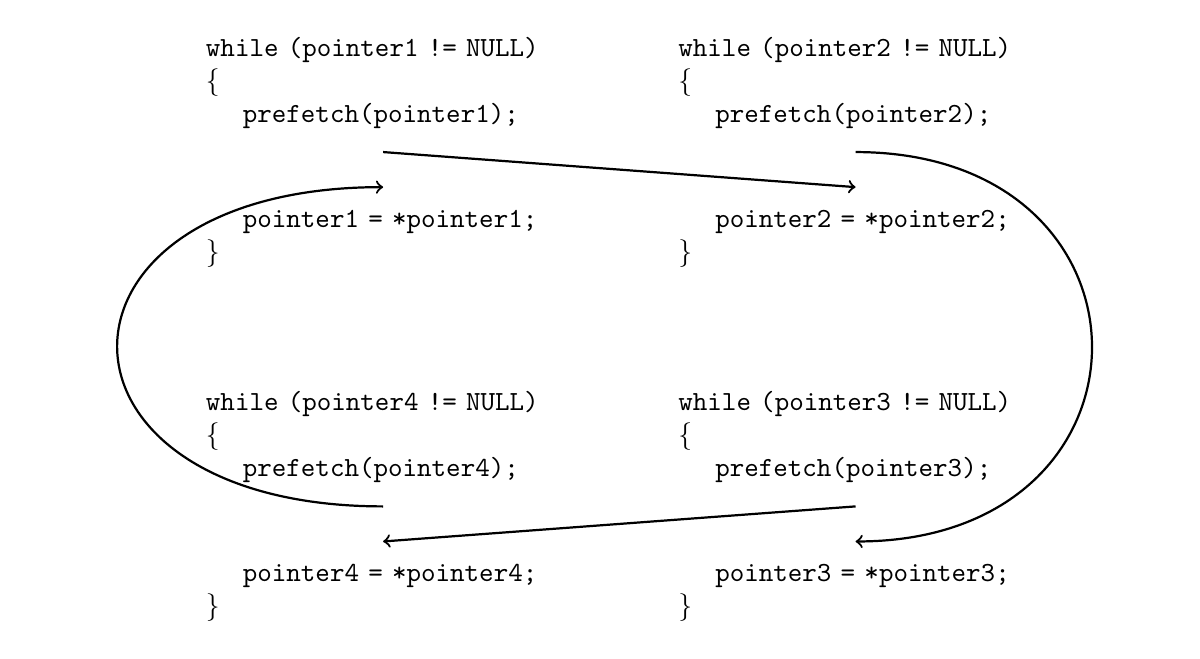
\begin{tikzpicture}[node distance=0.1cm]
  \node [,circle] (n1) at (0,0) { };
  \node [text width=4.5cm,above] at (n1.north) {
    \tt while (pointer1 != NULL) \{\\
    \ \ \ \ prefetch(pointer1);
  };
  \node [,circle] (s1) [below=of n1] { };
  \node [text width=4.5cm,below] at (s1.south) {
    \tt\ \ \ \ pointer1 = *pointer1;\\
    \}
  };

  \node [,circle] (n2) at (6,0) { };
  \node [text width=4.5cm,above] at (n2.north) {
    \tt while (pointer2 != NULL) \{\\
    \ \ \ \ prefetch(pointer2);
  };
  \node [,circle] (s2) [below=of n2] { };
  \node [text width=4.5cm,below] at (s2.south) {
    \tt\ \ \ \ pointer2 = *pointer2;\\
    \}
  };

  \node [,circle] (n3) at (6,-4.5) { };
  \node [text width=4.5cm,above] at (n3.north) {
    \tt while (pointer3 != NULL) \{\\
    \ \ \ \ prefetch(pointer3);
  };
  \node [,circle] (s3) [below=of n3] { };
  \node [text width=4.5cm,below] at (s3.south) {
    \tt\ \ \ \ pointer3 = *pointer3;\\
    \}
  };

  \node [,circle] (n4) at (0,-4.5) { };
  \node [text width=4.5cm,above] at (n4.north) {
    \tt while (pointer4 != NULL) \{\\
    \ \ \ \ prefetch(pointer4);
  };
  \node [,circle] (s4) [below=of n4] { };
  \node [text width=4.5cm,below] at (s4.south) {
    \tt\ \ \ \ pointer4 = *pointer4;\\
    \}
  };
 \draw[->, thick] (n1.center) -- (s2.center);
 \draw[->, thick] (n3.center) -- (s4.center);
 \draw[->, thick] (n2.center) .. controls +(right:4) and +(right:4)
 .. (s3.center);
 \draw[->, thick] (n4.center) .. controls +(left:4.5) and +(left:4.5) .. (s1.center);
\end{tikzpicture}
\end{document}
